% Chapter 10, Section 1

\section{Recurrent Neural Networks \difficultyInline{intermediate}}
\label{sec:rnns}

\subsection*{Intuition}

An RNN carries a running summary of the past—like a notepad you update after reading each word. This hidden state lets the model use prior context to influence current predictions. However, keeping reliable notes over long spans is hard: small errors can compound, and gradients may shrink or grow too much \cite{GoodfellowEtAl2016}.

\subsection*{Historical Context}

Early sequence models struggled with long-term dependencies due to vanishing gradients, motivating gated designs such as LSTM \cite{Hochreiter1997}. Practical training stabilized with techniques like gradient clipping and better initialization \cite{GoodfellowEtAl2016}.

% Index and glossary
\index{recurrent neural network}
\glsadd{recurrent-neural-network}

\subsection{Motivation}

Sequential data exhibits \emph{temporal dependencies} and \emph{order-sensitive} structure that cannot be modelled well by i.i.d. assumptions or fixed-size context windows alone \cite{GoodfellowEtAl2016,Prince2023,Bishop2006}. Time series data, such as energy load forecasting, financial returns, or physiological signals like ECG readings, inherently depend on the temporal order of observations, where past measurements directly influence future predictions. In natural language, the meaning of a word depends critically on its context within a sentence, as sentences conform to complex syntactic and discourse structures that unfold sequentially. Speech and audio processing similarly require temporal modelling, since phonemes combine sequentially to form words, and coarticulation effects span multiple frames, meaning the pronunciation of one sound is influenced by neighbouring sounds. Video understanding demands temporal reasoning as well, where actions unfold over time and temporal cues help disambiguate visually similar frames. Control and reinforcement learning present yet another domain where sequential processing is essential, as actions taken at one time step influence future observations, requiring the system to maintain memory of past states and decisions.

Classic feedforward networks assume fixed-size inputs and lack a persistent state, making them ill-suited for long-range dependencies. Recurrent architectures introduce a hidden state that acts as a compact, learned memory \index{memory!neural} and enables conditioning on arbitrary-length histories. Historically, recurrent ideas trace back to early neural sequence models and dynamical systems; practical training matured with BPTT \cite{Rumelhart1986} and later with gated units to mitigate vanishing/exploding gradients \cite{Hochreiter1997}. For further background see the RNN overview in \cite{GoodfellowEtAl2016} and educational treatments in \cite{D2LChapterRNN,WebRNNWikipedia,WebDLBRNN}.

\index{sequence modeling}\index{temporal dependency}\glsadd{recurrent-neural-network}

\subsection{Why Sequences Matter}

The unique value of sequence modelling stems from several fundamental capabilities that distinguish it from traditional approaches. Context awareness represents perhaps the most crucial aspect, as sequence models excel at understanding how earlier elements in a sequence systematically affect later ones, enabling them to capture dependencies that span across time or position. Variable-length handling is another essential feature, as these models can naturally work with inputs of any length without requiring padding or truncation, making them remarkably flexible for real-world data where sequence lengths vary unpredictably. The ability to capture temporal patterns—understanding how things change and evolve over time—provides sequence models with the power to model dynamic phenomena ranging from language structure to physical processes. Finally, these capabilities combine to enable natural interaction with machines, facilitating human-like communication through speech and text, which has revolutionised how we interface with technology in everyday life.

\subsection{Basic RNN Architecture}

An RNN maintains a hidden state $\vect{h}_t$ that evolves over time:

\begin{align}
\vect{h}_t &= \sigma(\mat{W}_{hh} \vect{h}_{t-1} + \mat{W}_{xh} \vect{x}_t + \vect{b}_h) \\
\vect{y}_t &= \mat{W}_{hy} \vect{h}_t + \vect{b}_y
\end{align}

where $\vect{x}_t$ is input at time $t$, and $\sigma$ is typically tanh.

\paragraph{Visual aid.} The following unrolled diagram shows shared parameters across time:
\begin{figure}[h]
    \centering
    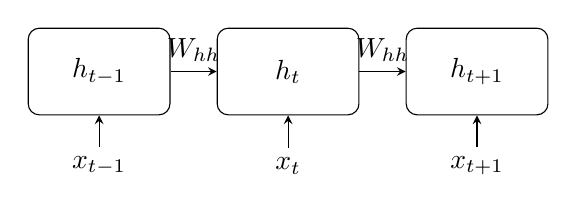
\begin{tikzpicture}[>=stealth, node distance=2.4cm]
        \tikzstyle{node}=[draw, rounded corners, minimum width=1.8cm, minimum height=1.1cm]
        \node[node] (h0) {$\vect{h}_{t-1}$};
        \node[node, right of=h0] (h1) {$\vect{h}_{t}$};
        \node[node, right of=h1] (h2) {$\vect{h}_{t+1}$};
        \draw[->] (h0) -- (h1) node[midway, above] {$\mat{W}_{hh}$};
        \draw[->] (h1) -- (h2) node[midway, above] {$\mat{W}_{hh}$};
        \node[below of=h0, yshift=1.2cm] (x0) {$\vect{x}_{t-1}$};
        \node[below of=h1, yshift=1.2cm] (x1) {$\vect{x}_{t}$};
        \node[below of=h2, yshift=1.2cm] (x2) {$\vect{x}_{t+1}$};
        \draw[->] (x0) -- (h0);
        \draw[->] (x1) -- (h1);
        \draw[->] (x2) -- (h2);
    \end{tikzpicture}
    \caption{Unrolled RNN with shared parameters across time steps.}
\end{figure}

\subsection{Unfolding in Time}

RNNs can be "unrolled" into a deep feedforward computation graph over time with \emph{shared parameters}. This perspective clarifies how gradients flow backward through temporal connections and why depth-in-time can cause vanishing/exploding gradients \cite{GoodfellowEtAl2016}.

\begin{equation}
\vect{h}_t = f(\vect{h}_{t-1}, \vect{x}_t; \vect{\theta})
\end{equation}

\paragraph{Visual aid.} Unfolding reveals repeated applications of the same transition function across steps. We annotate inputs, hidden states, and outputs to emphasize sharing and the temporal chain rule during BPTT.
\begin{figure}[h]
    \centering
    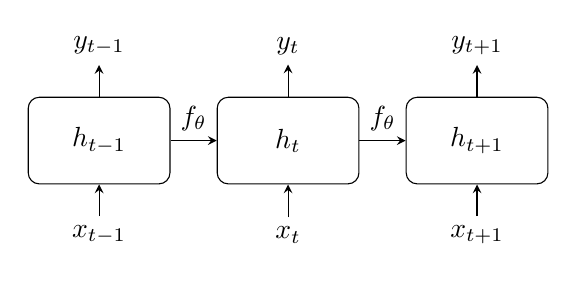
\begin{tikzpicture}[>=stealth, node distance=2.4cm]
        \tikzstyle{node}=[draw, rounded corners, minimum width=1.8cm, minimum height=1.1cm]
        \node[node] (h0) {$\vect{h}_{t-1}$};
        \node[node, right of=h0] (h1) {$\vect{h}_{t}$};
        \node[node, right of=h1] (h2) {$\vect{h}_{t+1}$};
        \draw[->] (h0) -- (h1) node[midway, above] {$f_{\vect{\theta}}$};
        \draw[->] (h1) -- (h2) node[midway, above] {$f_{\vect{\theta}}$};
        \node[below of=h0, yshift=1.2cm] (x0) {$\vect{x}_{t-1}$};
        \node[below of=h1, yshift=1.2cm] (x1) {$\vect{x}_{t}$};
        \node[below of=h2, yshift=1.2cm] (x2) {$\vect{x}_{t+1}$};
        \draw[->] (x0) -- (h0);
        \draw[->] (x1) -- (h1);
        \draw[->] (x2) -- (h2);
        \node[above of=h0, yshift=-1.2cm] (y0) {$\vect{y}_{t-1}$};
        \node[above of=h1, yshift=-1.2cm] (y1) {$\vect{y}_{t}$};
        \node[above of=h2, yshift=-1.2cm] (y2) {$\vect{y}_{t+1}$};
        \draw[->] (h0) -- (y0);
        \draw[->] (h1) -- (y1);
        \draw[->] (h2) -- (y2);
    \end{tikzpicture}
    \caption{Unrolling an RNN across time: the same parameters $\vect{\theta}$ are reused at each step.}
\end{figure}

This view connects RNNs to dynamic Bayesian networks and emphasizes that training complexity scales with the unroll length. See \cite{WebRNNWikipedia,GoodfellowEtAl2016,D2LChapterRNN}.

\index{unrolling in time}\index{shared parameters}

\subsection{Types of Sequences}

\begin{table}[h]
\centering
\begin{tabular}{|l|p{0.5\textwidth}|p{0.3\textwidth}|}
\hline
\textbf{Type} & \textbf{Description} & \textbf{Examples} \\
\hline
One-to-one & Fixed-size input to fixed-size output with temporal structure ignored or not present & Static image classification \\
\hline
One-to-many & Single input to sequence output & Image captioning \\
\hline
Many-to-one & Sequence input to single output & Sentiment classification; keyword spotting \\
\hline
Many-to-many (synchronous) & Sequence labeling with aligned input/output lengths & Part-of-speech tagging; frame labeling \\
\hline
Many-to-many (asynchronous) & Sequence transduction with potentially different lengths. Attention helps bridge length mismatch by learning soft alignments \cite{Bahdanau2014} & Machine translation; speech recognition \\
\hline
\end{tabular}
\caption{Types of sequence models and their characteristics.}
\label{tab:sequence-types}
\end{table}

Design choices (teacher forcing, bidirectionality, attention, beam search) depend on whether future context is available and whether output timing must be causal. See \cite{D2LChapterRNN,WebRNNWikipedia} for further taxonomy.

\index{sequence types}\index{sequence labeling}\index{sequence transduction}

% Citations
See \cite{GoodfellowEtAl2016,Prince2023,Bishop2006,WebRNNWikipedia,WebDLBRNN,D2LChapterRNN} for introductions to sequence modeling and RNNs.

